\section{Computations}\label{sec:numerics}

\subsection{Code and meshes}
Except in Section~\ref{sec:numv3}, we use $P_4$ Scott--Vogelius elements with Nitsche's method on the inscribed polygon and strong Dirichlet data on the square $R=(-2.5,2.5)^2$. Divergence is enforced exactly: all ten $P_3$ moments per triangle.

Saddle-point systems are solved by SuperLU \cite{SuperLU} with partial pivoting and three steps of iterative refinement. Over the $148$ production solves ($74$ cases, two methods each), the relative residual is at most $3.8\cdot10^{-15}$ and the discrete divergence at most $7\cdot10^{-11}$ (median $9\cdot10^{-12}$).

For the zero-pressure-gradient benchmark of \cite{Cavalcante}, the code gives the coercivity threshold $\mu^\ast=60.343$ at $N=20$ (\texttt{results/pod/thresh/}\allowbreak\texttt{N20\_L2.5\_m5.json}), against the transition $60.33821<\mu^\ast<60.33831$ reported there.

The vertices of $\Gh$ are the radial projections of $N$ equispaced points on the square, so the boundary chords are \emph{not} equal (except for $N=8$): $\max|e|/\min|e|$ is $1.43$, $1.72$, $1.87$ and $1.97$ at $N=16$, $32$, $64$ and $256$. The ratio $h/\hG=\hO/\max|e|$ stays in $3.28$--$3.48$, while $\rho=h/\min|e|$ of Section~\ref{sec:setting} is $4.70$, $5.73$ and $6.35$ at $N=16$, $32$ and $64$. $\hO$ decreases from $1.505$ to $0.109$ for $N=16\to256$; since $h/\hG$ is nearly constant, rates in $\hO$ and $\hG$ coincide. Penalty thresholds are reported as $\gamma^\ast=\mu^\ast\hG/h$, which is the $\gamma$ of Section~\ref{sec:setting}. Rates in the tables are computed between consecutive runs of the full sequence $N=16,24,32,48,64,96,128,192,256$, some of which are omitted from the tables.

\emph{The production penalty.} Most runs use $\mu=100$, i.e.\ $\gamma\approx29$--$30$. This is only $1.37$--$1.41$ times the measured coercivity threshold on $\Zh$ ($\mu^\ast=50.3\to70.7$ for $N=8\to64$, extrapolated limit $\approx73$; Table~\ref{tab:thresh}). For $\CNS$, which is Petrov--Galerkin on $\Zh$, the relevant quantity is the largest $\mu$ at which the square system is singular: $\mu_c^{\CNS}=78.9,84.4,88.1$ at $N=16,32,64$, extrapolating to about $93$ ($\gamma_c\approx26.5$). So $\mu=100$ is stable for $\CNS$ on every production mesh, but the margin shrinks from $27\%$ ($N=16$) to $19\%$ ($N=32$) and $13\%$ ($N=64$), and to about $7\%$ as $h\to0$; the critical mode is about $99\%$ normal and edge-mean dominated, unlike the tangential $\GS$ mode (Remark~\ref{rb:rem:mu100}). The thresholds $\gamma_0,\gamma_2$ required by the proofs are not computed, so the $\mu=100$ runs illustrate the theorems rather than being covered by them. Near the threshold the discrete solution is amplified by a factor of order $(1-\mu^\ast(N)/\mu)^{-1}$, which drifts from about $2.5$ to $3.4$ over $N=16\to64$; on its own this can lower measured rates by up to about $0.2$ per doubling at $N\le64$. Normalised constants that should tend to $1$ or to a limit (slip ratios, drag ratios, $H^1$ constants) are therefore partly pre-asymptotic at $\mu=100$; where $\mu=300$, $10^3$ or $10^4$ data exist we quote them alongside (Tables~\ref{tab:P}, \ref{tab:Pv3}).

\subsection{Test problems}
\begin{itemize}
\item[\textbf{A}] Scott's benchmark: the shear flow $u=(1-r^{-2})(-y,x)$ with $p\equiv0$, so $G=0$.
\item[\textbf{B$_a$}] $\psi=(r^2-1)^2(x+y^2/2)/10$ and $p=a(x^2y-y+x/2)$, so $G=a(7\pi/8)^{1/2}$: $G=1.658$ for $a=1$ and $165.8$ for $a=100$.
\item[\textbf{P}] Pure pressure: $u\equiv0$, $f=\nabla p$, with $p$ as in B$_1$. $\CNS$ reproduces this exactly ($u_h=0$ and $p_h=p-\pbG(p)$, since $p\in\Pih$); its computed velocity is below $10^{-13}$ in $H^1$. The $\GS$ output is therefore \emph{exactly} the response to the missing traction.
\item[\textbf{C}] $\psi$ as in B, with the non-polynomial pressure $p=e^{x/2}\cos y$. This exercises the term $p^\ast-\pi_hp^\ast$ of Theorem~\ref{thm:D}.
\end{itemize}
Tests A and B were run with $\mu\in\{100,1000,10000\}$ and $N\le192$, plus $N=256$ for $(A,100)$ and $(B_1,100)$, on a 32-core machine (36 minutes in total). Test P (all three $\mu$) and test C ($\mu=100$) were run with $N\le96$ on a 2-core machine.

\begin{figure}[t]
\centering
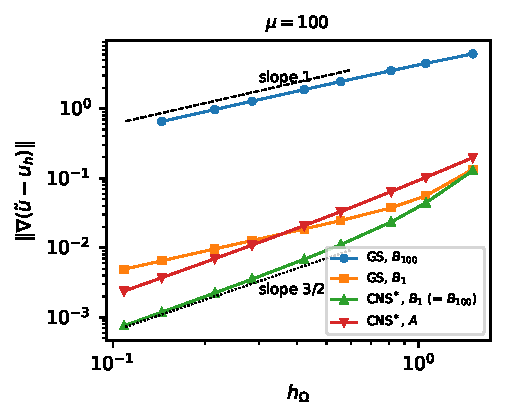
\includegraphics[width=0.48\textwidth]{figures/h1_rates.pdf}\hfill
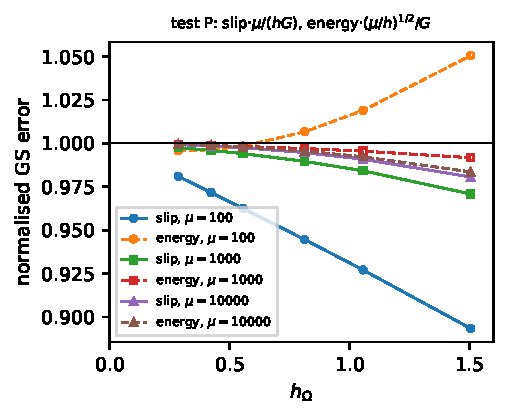
\includegraphics[width=0.48\textwidth]{figures/leading_term.pdf}
\caption{Left: $H^1$ errors at $\mu=100$. Once $G>0$, $\GS$ eventually has slope $1$, while $\CNS$ tends to slope $3/2$ independently of the pressure. Right: the normalised slip and energy errors of $\GS$ on test P approach $1$ (Corollary~\ref{cor:Bp}); at $N=96$ the energy ratios are within $0.5\%$ of $1$ and the slip ratios within $2\%$.}
\label{fig:rates}
\end{figure}

\begin{table}[t]
\centering
\caption{$\CNS$ attains Scott's rate $\hG^{3/2}$ (Theorem~\ref{thm:D}). $H^1$ error, $\mu=100$.}\label{tab:cns}
\begin{tabular}{rrcccc}
\toprule
$N$ & $\hO$ & A & rate & B$_1$ & rate\\
\midrule
32 & 0.813 & $6.41\cdot10^{-2}$ & 1.80 & $2.34\cdot10^{-2}$ & 2.43\\
64 & 0.422 & $2.08\cdot10^{-2}$ & 1.69 & $6.83\cdot10^{-3}$ & 1.76\\
96 & 0.285 & $1.09\cdot10^{-2}$ & 1.64 & $3.54\cdot10^{-3}$ & 1.68\\
128 & 0.215 & $6.96\cdot10^{-3}$ & 1.60 & $2.24\cdot10^{-3}$ & 1.63\\
192 & 0.144 & $3.71\cdot10^{-3}$ & 1.58 & $1.19\cdot10^{-3}$ & 1.60\\
256 & 0.109 & $2.39\cdot10^{-3}$ & 1.56 & $7.58\cdot10^{-4}$ & 1.57\\
\bottomrule
\end{tabular}
\end{table}

\subsection{Theorem~\ref{thm:D}: $\CNS$}
Table~\ref{tab:cns} gives the $\CNS$ errors. At $N=256$ the energy-norm rate is $1.52$ and the slip rate is $2.02$; the slip carries an extra factor $(h/\mu)^{1/2}$. The $H^1$ rates decrease monotonically toward $3/2$, the geometric term of Lemma~\ref{lem:transposed}. The $\hO^4$ term is invisible at these levels because the geometric term dominates.

The error is independent of the pressure.
\begin{itemize}
\item For polynomial pressures this is structural ($p\in\Pih$). B$_1$ and B$_{100}$ agree to all printed digits wherever both were run ($N\le192$, every $\mu$).
\item With the non-polynomial pressure of test C, the $\CNS$ $H^1$ error differs from that of B$_1$ by a relative $7.9\cdot10^{-7}$, $3.9\cdot10^{-8}$ and $9.7\cdot10^{-9}$ at $N=16$, $64$ and $96$. This is the size of the contribution $\ip{p^\ast-\pi_hp^\ast}{v\cdot n}$, which is of higher order, as Theorem~\ref{thm:D} predicts.
\end{itemize}

\subsection{Theorems~\ref{thm:A}--\ref{thm:C}: the printed method}
Table~\ref{tab:gs} compares the $H^1$ rates of $\GS$ and $\CNS$ on B$_{100}$.

For the non-polynomial test C at $\mu=100$, the $\GS$ $H^1$ rate from $N=64$ to $96$ is already $1.12$, against $1.68$ for $\CNS$. For the small pressure B$_1$ at $\mu=1000$, $\GS$ still shows $1.51$ at $N=192$. The $(h/\mu)G$ term dominates only once $(h/\mu)G\gtrsim\hG^{3/2}$, which always happens eventually because $\hG^{3/2}$ decays faster. Larger $\mu$ or smaller $G$ delays the crossover but does not remove it.

\begin{table}[t]
\centering
\caption{$\GS$ eventually loses Scott's rate once $G>0$. $H^1$ rate between $N=128$ and $N=192$, test B$_{100}$.}\label{tab:gs}
\begin{tabular}{rcc}
\toprule
$\mu$ & $\GS$ & $\CNS$\\
\midrule
100 & 0.99 & 1.60\\
1000 & 1.00 & 1.56\\
10000 & 1.06 & 1.58\\
\bottomrule
\end{tabular}
\end{table}

\subsection{Corollary~\ref{cor:Bp}: the leading term}
Table~\ref{tab:P} and Figure~\ref{fig:rates} (right) show the normalised $\GS$ error on test P, and Figure~\ref{fig:leak} shows the leak field itself.
\begin{itemize}
\item At $N=32$, $\mu=100$, the normal trace of $u_h$ on $\Gh$ matches the prediction $(h/\mu)(p-\pbar)$ with relative $L^2(\Gh)$ misfit $0.055$. The maximum of the tangential trace is about $12\%$ of that of the normal one, and the tangential trace oscillates at the element scale.
\item The slip and energy ratios approach $1$: at $N=96$ the energy ratios are within $0.5\%$ of $1$ for every $\mu$. The defect in the slip ratio shrinks with $h/\mu$: at $N=96$ it is $0.019$, $0.0025$ and $0.0007$ for $\mu=10^2$, $10^3$ and $10^4$.
\item The $H^1$ constant is not covered by the corollary. For $\mu=100$ it rises from $2.46$ to $2.71$; for $\mu=10^3$ and $10^4$ it falls, from $2.78$ to $2.77$ and from $3.06$ to $2.79$. Section~\ref{hc:sec} identifies the limit as $K=\norm{\nabla U}/G=2.7565$ for this box, proves convergence to it as $h\to0$ at fixed $\mu$ (Corollary~\ref{hc:cor}; on these meshes $h/\hG$ is nearly constant, so fixed $\mu$ means fixed $\gamma$ and bounded $\rho$), and compares it pointwise with these runs. The $\mu=100$ values approach it from below; the larger-$\mu$ values approach it from above, in the regime $\gamma\hG\gg1$, which Corollary~\ref{u:Kall} covers: on test P, $|K_h-K|\le C(\hG+(E^0_U)^2)$ for every penalty.
\item On test B, $\GS$ itself (B$_1$, $\mu=100$, $N=256$) gives slip and energy ratios $0.995$ and $1.001$.
\item For $\mu=10^4$ with the small pressure B$_1$, $\gamma\hG\approx120\gg G$ at $N=192$, so the hypothesis of the corollary fails. The $\GS$ energy ratio there is about $7.8$, dominated by the geometric error rather than the traction response.
\item The difference $u_{\GS}-u_{\CNS}$ is not a clean proxy for the traction response on test B. It also contains the difference between the two methods on the velocity part, which is $O(\hG^{3/2})$ and non-zero even for test A. Test P removes this.
\end{itemize}

\begin{figure}[t]
\centering
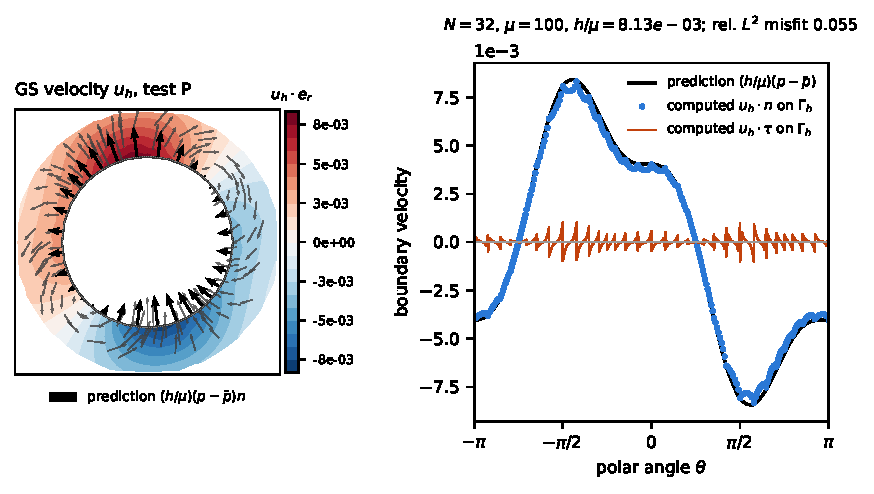
\includegraphics[width=\textwidth]{figures/leak_field.pdf}
\caption{The leak of the printed method on test P ($u=0$, so $u_h=-(\ut-u_h)$), $N=32$, $\mu=100$. Left: radial velocity $u_h\cdot e_r$ near the wall (colour) and $u_h$ (thin arrows); thick arrows show the prediction $(h/\mu)(p-\pbar)n$ of Corollary~\ref{cor:Bp} at the chord midpoints. Right: normal and tangential traces of $u_h$ along $\Gh$ against $(h/\mu)(p-\pbar)$.}
\label{fig:leak}
\end{figure}

\begin{table}[t]
\centering
\caption{The leading term of Corollary~\ref{cor:Bp}. Normalised $\GS$ error on test P ($G=1.658$), where $e=\ut-u_h$.}\label{tab:P}
\begin{tabular}{rrccc}
\toprule
$N$ & $\mu$ & $\norm{\nabla e}\,\mu/(hG)$ & $\norm{e}_{\Gh}\,\mu/(hG)$ & $\tnorm{e}(\mu/h)^{1/2}/G$\\
\midrule
16 & 100 & 2.464 & 0.893 & 1.050\\
32 & 100 & 2.612 & 0.945 & 1.007\\
64 & 100 & 2.684 & 0.972 & 0.996\\
96 & 100 & 2.708 & 0.981 & 0.996\\
96 & 1000 & 2.770 & 0.998 & 0.999\\
96 & 10000 & 2.790 & 0.9993 & 0.9994\\
\bottomrule
\end{tabular}
\end{table}

\subsection{Proposition~\ref{prop:penalty}: the penalty study}
The coercivity threshold $\mu^\ast$ on $\Zh$ is the smallest $\mu$ for which the unpivoted symmetric factorisation of $A_\mu+rB^{\mathsf T}M^{-1}B$ has only positive pivots; we locate it by bisection. Table~\ref{tab:thresh} and Figure~\ref{fig:thresh} show the results.

Under refinement at fixed $h/\hG$, $\gamma^\ast$ increases by $3.4$ ($N=8\to16$), $1.8$ ($16\to32$) and $0.95$ ($32\to64$). The increments roughly halve. The limit is the threshold of a periodic half-plane cell (Proposition~\ref{pb:gamlim}): $\gamma^\ast_\infty=21.408$ at full depth, $21.4045$ for fields in the first two layers, and the two-layer global thresholds for $N=128,\dots,2048$ extrapolate to $21.40452$, with $\gamma^\ast(N)\approx\gamma^\ast_\infty-22/N$.

In part (b) of Table~\ref{tab:thresh}, $h/\hG$ is varied by coarsening the far field while the vertices of $\Gh$ are held fixed and the boundary layer approximately fixed. Then $\mu^\ast$ is linear in $h/\hG$ over more than a decade, with a constant slope of about $18$--$20$. The vertices of $\Gh$ do not depend on $L$, so $\max|e|/\min|e|$ is fixed at fixed $N$, and $\mu^\ast$ is equally linear in $\rho$, with the slope divided by that ratio. The threshold is thus set locally at $\Gh$ ($\mu/h\gtrsim c/\hG$), and the scaling with $h/\hG$ (hence with $\rho$) is the cost of normalising the penalty by the global $h$.

In practical terms:
\begin{itemize}
\item for $k=4$ a safe choice is $\gamma=\mu\hG/h\ge25$, that is, $\mu\ge25\,h/\hG$; since $\rho\ge h/\hG$, $\mu\ge25\rho$ is also safe;
\item a fixed $\mu$ fails once the far field is coarsened beyond $h/\hG\approx\mu/20$;
\item the threshold grows quickly with $k$, and is larger on Clough--Tocher refinements (Section~\ref{sec:numv3}), so these values do not transfer to other elements.
\end{itemize}
The exact certificate $\lambda\ge9$ on $\cS_3$ and $\cS_4'$ is a local lower bound, consistent with the global $\gamma^\ast\approx18$--$21$; Section~\ref{pb:sec} accounts for the gap.

\begin{table}[t]
\centering
\caption{Coercivity threshold $\mu^\ast$ and $\gamma^\ast=\mu^\ast\hG/h$ ($k=4$). The row $h/\hG$ is $\hO/\max|e|$; the $\rho=h/\min|e|$ of Section~\ref{sec:setting} is larger by the factor $\max|e|/\min|e|$ (for example $\rho=4.70$, $5.73$, $6.35$ at $N=16$, $32$, $64$ in part (a)).}\label{tab:thresh}
\small
\textit{(a) Refinement at fixed $h/\hG\approx3.3$.}\\[2pt]
\begin{tabular}{lcccccccc}
\toprule
$N$ & 8 & 12 & 16 & 20 & 24 & 32 & 48 & 64\\
\midrule
$h/\hG$ & 3.41 & 3.02 & 3.28 & 3.16 & 3.30 & 3.33 & 3.37 & 3.40\\
$\rho$ & 3.41 & 4.16 & 4.70 & 5.08 & 5.36 & 5.73 & 6.13 & 6.35\\
$\mu^\ast$ & 50.3 & 51.8 & 59.3 & 60.3 & 63.3 & 66.0 & 69.1 & 70.7\\
$\gamma^\ast$ & 14.7 & 17.1 & 18.1 & 19.1 & 19.2 & 19.9 & 20.5 & 20.8\\
\bottomrule
\end{tabular}\\[6pt]
\textit{(b) Varying $h/\hG$ through the outer box $(-L,L)^2$.}\\[2pt]
\begin{tabular}{llccccc}
\toprule
 & $L$ & 2.5 & 5 & 10 & 20 & 40\\
\midrule
$N=16$ & $h/\hG$ & 3.28 & 5.90 & 11.3 & 22.2 & 43.9\\
 & $\mu^\ast$ & 59.3 & 112.1 & 208.0 & 411.5 & 809.3\\
 & $\gamma^\ast$ & 18.1 & 19.0 & 18.4 & 18.5 & 18.4\\
\midrule
$N=32$ & $h/\hG$ & 3.33 & 5.79 & 10.8 & 21.1 & 41.5\\
 & $\mu^\ast$ & 66.0 & 113.9 & 218.0 & 422.2 & 835.7\\
 & $\gamma^\ast$ & 19.9 & 19.7 & 20.1 & 20.0 & 20.1\\
\bottomrule
\end{tabular}
\end{table}

\begin{figure}[t]
\centering
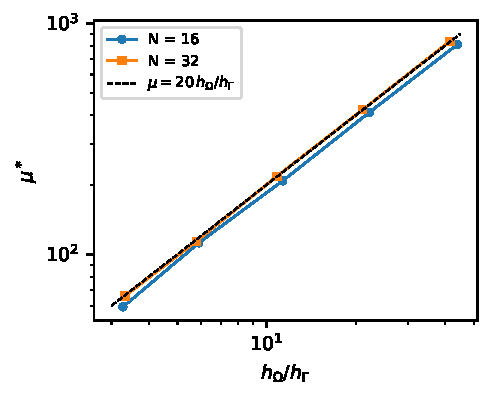
\includegraphics[width=0.48\textwidth]{figures/threshold.pdf}
\caption{Coercivity threshold $\mu^\ast$ against $h/\hG$ (Table~\ref{tab:thresh}(b)).}
\label{fig:thresh}
\end{figure}

\subsection{Lemma tests}
We compute exact discrete dual norms, $\sup_v\ell(v)/\norm{\nabla v}$ over $\Zh$ or $\VR$, by a saddle-point solve with the pointwise divergence constraint. Table~\ref{tab:lemma} gives the rates for $N=48\to64$.
\cert{code/lemma\_tests.py 16,24,32,48,64}{logs/lemma\_tests.log}

\begin{table}[t]
\centering
\caption{Exact discrete dual norms; rate in $\hG$ for $N=48\to64$ (positive means decay).}\label{tab:lemma}
\begin{tabular}{llc}
\toprule
Functional & Space & Rate\\
\midrule
$\ip{S}{\dn v}$, $S$ normal & $\Zh$ & $+0.05$ (bounded, $\approx1.75$)\\
$\ip{S}{\dn v}$, $S$ normal & $\VR$ & $-0.52$\\
$\ip{S}{\dn v}$, $S$ tangential & $\Zh$ & $-0.52$\\
$\ip{(\nabla\ut)^{\mathsf T}n}{v}$, tests A / B & $\VR$ & $1.57$ / $1.56$ (Lemma~\ref{lem:transposed}: $3/2$)\\
\bottomrule
\end{tabular}
\end{table}


\subsection{Strong imposition and the \texorpdfstring{$h^{1/2}$}{h^(1/2)} phenomenon}\label{num:strong}
Table~\ref{tab:strong} compares strongly imposed no-slip, $u_h=0$ at every node of $\Gh$ with no Nitsche terms and the same $P_4$--$P_3^{\rm disc}$ pair, with $\GS$ and $\CNS$ on test A.
\cert{code/strong\_bc.py; code/report\_v5.py}{results/v5/strong/, results/v5/letter\_tables.txt (T1, T1$'$)}
\begin{itemize}
\item \emph{Mesh (a): the rate $h^{1/2}$ is reproduced.} On mesh (a) the first-layer diagonals alternate, so every other polygon vertex lies in only two triangles. The $H^1$ rate of strong imposition falls from $0.75$ to $0.56$ at $N=128$, towards $\frac12$. The largest vertex-gradient error $\max_{z,T\ni z}|\nabla u_h|_T(z)-\nabla u(z)|$ tends to $1.99$, which is $|\dn u\cdot\tau|=2$ at $r=1$ for this flow: the discrete gradient vanishes at those vertices. The pressure norm grows like $h^{-1/2}$ ($\norm{p_h}=14.0\to35.7$, although $p\equiv0$).
\item \emph{Mesh (s): no locking in the range computed.} On the mesh of the rest of this section every polygon vertex lies in three triangles. Strong imposition then converges with $H^1$ rates $1.93\to1.61$ ($N=24\to128$), like the Nitsche methods and with an error about $2.5$ times larger; the vertex-gradient error decays like $h$ ($1.28\to0.16$), and $\norm{p_h}$ decays. Imposing $u_h=\ut$ at the nodes of $\Gh$ instead of $u_h=0$ gives rate $\approx4$, so the defect of strong imposition is entirely the transfer of the no-slip value $u=0$ from $\Gamma$ to $\Gh$.
\item \emph{$\GS$ and $\CNS$ do not see the change of mesh.} On mesh (a) their $H^1$ errors at $N=128$ are $6.00\cdot10^{-3}$ and $7.17\cdot10^{-3}$, against $6.11\cdot10^{-3}$ and $6.96\cdot10^{-3}$ on mesh (s); at every $N\le128$ the two meshes differ by at most $6\%$.
\end{itemize}
\begin{remark}[How to read Table~\ref{tab:strong}]\label{num:rem:strong}
Section~\ref{st:sec} explains these observations. On mesh (s) (M2) holds, and strong imposition has $H^1$ error $\asymp\hG^{3/2}$ (Corollary~\ref{st:two0}); the slow drift of the observed rate ($1.547$ at $N=192$) is a relative $O(\hG)$ correction, $E\approx a\hG^{3/2}(1+\beta\hG)$ with $\beta\approx1.1$--$1.3$ (Table~\ref{st:tab:drift}). The vertex-gradient error $\asymp h$ is exactly $a_z|e|/2$ on each chord (Lemma~\ref{st:P1}). On mesh (a) every other wall vertex is locked (two triangles), and the error is $\asymp\hG^{3/2}+\hG(\sum_{\Lk}a_z^2)^{1/2}\asymp\hG^{1/2}$ (Corollary~\ref{st:two}); the counting lower bound of Theorem~\ref{st:S3} is within a factor $3.0$--$3.15$ of the measured error. A single locked vertex already gives rate $1$, and nearly singular three-triangle stars give rates between $\frac32$ and $\frac12$ according to the needle angle (Section~\ref{st:sec:ns}). Mesh (a) violates (M1$'$) and (M2) at its two-triangle vertices, so it lies outside the hypotheses of our theorems for $\GS$ and $\CNS$; that these methods are unaffected on it is an observation. So the zero-gradient defect of strong imposition is a property of the wall mesh, and under (M2) the advantage of weak imposition is a smaller constant (about $2.5$ here), not a better rate.
\end{remark}
\begin{table}[t]
\centering
\caption{Strong imposition against Nitsche. Test A, $k=4$, $\mu=100$: $H^1$ seminorm error $|\ut-u_h|_{1,\Oh}$. \emph{Strong}: $u_h=0$ at all nodes of $\Gh$, no Nitsche terms, on mesh (s), the mesh of Section~\ref{sec:numerics} (every polygon vertex in three triangles), and on mesh (a), the same mesh with alternating first-layer diagonals (polygon vertices in two or four triangles). $\GS$ and $\CNS$ on mesh (s).}\label{tab:strong}
\small
\begin{tabular}{rrrrrrrrrr}
\toprule
$N$ & $h$ & \multicolumn{2}{c}{strong, mesh (a)} & \multicolumn{2}{c}{strong, mesh (s)} & \multicolumn{2}{c}{$\GS$} & \multicolumn{2}{c}{$\CNS$}\\
\cmidrule(lr){3-4} \cmidrule(lr){5-6} \cmidrule(lr){7-8} \cmidrule(lr){9-10}
 & & error & rate & error & rate & error & rate & error & rate\\
\midrule
16 & 1.5052 & $9.03\cdot10^{-1}$ & -- & $4.62\cdot10^{-1}$ & -- & $1.72\cdot10^{-1}$ & -- & $1.98\cdot10^{-1}$ & --\\
24 & 1.0559 & $6.91\cdot10^{-1}$ & 0.75 & $2.33\cdot10^{-1}$ & 1.93 & $8.87\cdot10^{-2}$ & 1.86 & $1.03\cdot10^{-1}$ & 1.85\\
32 & 0.8127 & $5.72\cdot10^{-1}$ & 0.72 & $1.43\cdot10^{-1}$ & 1.86 & $5.55\cdot10^{-2}$ & 1.79 & $6.41\cdot10^{-2}$ & 1.80\\
48 & 0.5560 & $4.44\cdot10^{-1}$ & 0.67 & $7.29\cdot10^{-2}$ & 1.78 & $2.88\cdot10^{-2}$ & 1.73 & $3.31\cdot10^{-2}$ & 1.74\\
64 & 0.4224 & $3.75\cdot10^{-1}$ & 0.62 & $4.56\cdot10^{-2}$ & 1.71 & $1.81\cdot10^{-2}$ & 1.68 & $2.08\cdot10^{-2}$ & 1.69\\
96 & 0.2853 & $2.98\cdot10^{-1}$ & 0.59 & $2.38\cdot10^{-2}$ & 1.65 & $9.57\cdot10^{-3}$ & 1.63 & $1.09\cdot10^{-2}$ & 1.64\\
128 & 0.2153 & $2.54\cdot10^{-1}$ & 0.56 & $1.52\cdot10^{-2}$ & 1.61 & $6.11\cdot10^{-3}$ & 1.59 & $6.96\cdot10^{-3}$ & 1.60\\
192 & 0.1445 & -- & -- & -- & -- & $3.27\cdot10^{-3}$ & 1.57 & $3.71\cdot10^{-3}$ & 1.58\\
256 & 0.1087 & -- & -- & -- & -- & $2.10\cdot10^{-3}$ & 1.55 & $2.38\cdot10^{-3}$ & 1.56\\
\bottomrule
\end{tabular}
\end{table}

\subsection{Pressure errors, stress and drag}\label{pd:sec:num}
All runs use $k=4$ and $\mu=100$, and measure $\norm{p^\circ-p_h}_{L^2(\Oh)}$ with $p^\circ=\pt-\pbG(\pt)$, the target of Theorems~\ref{pd:thm:cnsp} and~\ref{pd:thm:gsp}, for both methods. Removing the optimal constant instead changes these errors in the third digit at most; the discrete pressures are thus $\pbG$-normalised up to a vanishing constant, even though $\pbG(p_h)\ne0$ ($\pbG(p_h)=-4.6\cdot10^{-3}\to-9.7\cdot10^{-4}$ for $\CNS$ on B$_1$, $N=16\to96$). The velocity $H^1$ errors of these runs reproduce the stored ones to a relative $2.1\cdot10^{-7}$. The results are in Tables~\ref{tab:B100}--\ref{tab:pA}.
\cert{code/pressure\_err.py; code/report\_v5.py}{results/v5/pressure/, results/v5/letter\_tables.txt (T2, T4)}
\begin{itemize}
\item \emph{$\CNS$.} The pressure error does not depend on the pressure data: for B$_1$, B$_{100}$ and C it agrees to $10^{-6}$ at $N=16$ and $3\cdot10^{-11}$ at $N=96$. Its $L^2$ rates $3.0,3.0,2.6,2.1,1.8$ decrease towards $\frac32$, as Theorem~\ref{pd:thm:cnsp} predicts; the first-layer part already has rate about $1.6$, and the $L^\infty$ error on the first layer has rate about $1$ ($0.98$ at $N=96$), for which we have no proof.
\item \emph{$\GS$ with $G>0$.} The $L^2$ rate decreases towards $\frac12$ ($0.60$, $0.62$, $0.63$ at $N=96$ for B$_1$, B$_{100}$, C). The first-layer part has rate $0.48$--$0.50$ and the rest rate $0.9$--$1.0$; the $L^\infty$ error on the first layer does not converge ($0.78$ for B$_1$, $77$ for B$_{100}$). This is Theorem~\ref{pd:thm:gsp}. For B$_{100}$ the $\GS$ pressure error is $9.2$ at $N=96$, against $8\cdot10^{-3}$ for $\CNS$.
\item \emph{$\GS$ with $G=0$} (test A) behaves like $\CNS$: $L^2$ rate $1.68$ at $N=96$ and still decreasing, and the first layer converges.
\end{itemize}
\emph{Layer, drag and traction.} On test P with $\GS$ at $N=64$ and $96$, the first-layer pressure error is $0.0958$ and $0.0793$, against $\norm{\xib}=0.0961$ and $0.0796$ from Definition~\ref{pd:def:xib}; the rest is $0.069$ and $0.047$. The Nitsche-flux drag defect $J^N_h-J_{e_1}+\Theta_f$ is $0.970$ and $0.981$ times the prediction $-(h/\mu)K_{e_1}$ of Theorem~\ref{pd:thm:gsdrag} ($K_{e_1}\approx17.16$, $K_{e_2}\approx-25.36$); for Gjerde--Scott's volume formula the ratio to $-2(h/\mu)K_{e_1}$ is $0.905$ and $0.952$ at $N=32$ and $64$ (Proposition~\ref{pd:prop:chi}). The pointwise-traction drag error does not converge: $J^\beta_h-J_{e_1}=-1.211$ and $-1.225$ at $N=64$ and $96$, against $\Xi_h=-1.192$ at $N=64$ (Proposition~\ref{pd:prop:beta}). For $\CNS$ on B$_1$, the lift defect divided by $-\Theta_f-\Lambda_h$ is $0.788,0.895,0.941,0.955$ for $N=16$--$96$, and on test A the torque ratio is $0.84,0.92,0.95$ (Theorem~\ref{pd:thm:cnsdrag}). At fixed $N=64$ the $\CNS$ pressure error on B$_1$ grows with the penalty ($0.016$, $0.039$, $0.059$ for $\mu=10^2,10^3,10^4$), which is the non-uniformity in $\gamma$ of Remark~\ref{pd:rem:cnsp}.
\cert{notes/v4/pressure\_drag\_check.py}{notes/v4/pressure\_drag\_report.md, Section~3 (no log file)}
\begin{table}[t]
\centering
\caption{Test B$_{100}$ (large pressure variation, $p=100(x^2y-y+x/2)$), $k=4$, $\mu=100$: velocity error $|\ut-u_h|_{1,\Oh}$ and pressure error $\norm{p^\circ-p_h}_{L^2(\Oh)}$, $p^\circ=\pt-\pbG(\pt)$.}\label{tab:B100}
\small
\begin{tabular}{rrrrrrrrrr}
\toprule
$N$ & $h$ & \multicolumn{2}{c}{$\GS$, $|\cdot|_1$} & \multicolumn{2}{c}{$\CNS$, $|\cdot|_1$} & \multicolumn{2}{c}{$\GS$, $L^2$ pressure} & \multicolumn{2}{c}{$\CNS$, $L^2$ pressure}\\
\cmidrule(lr){3-4} \cmidrule(lr){5-6} \cmidrule(lr){7-8} \cmidrule(lr){9-10}
 & & error & rate & error & rate & error & rate & error & rate\\
\midrule
16 & 1.5052 & $6.14$ & -- & $1.29\cdot10^{-1}$ & -- & $2.75\cdot10^{1}$ & -- & $4.97\cdot10^{-1}$ & --\\
24 & 1.0559 & $4.48$ & 0.89 & $4.42\cdot10^{-2}$ & 3.02 & $2.17\cdot10^{1}$ & 0.67 & $1.69\cdot10^{-1}$ & 3.04\\
32 & 0.8127 & $3.51$ & 0.93 & $2.34\cdot10^{-2}$ & 2.43 & $1.82\cdot10^{1}$ & 0.68 & $7.67\cdot10^{-2}$ & 3.03\\
48 & 0.5560 & $2.45$ & 0.95 & $1.11\cdot10^{-2}$ & 1.97 & $1.41\cdot10^{1}$ & 0.67 & $2.87\cdot10^{-2}$ & 2.59\\
64 & 0.4224 & $1.88$ & 0.97 & $6.83\cdot10^{-3}$ & 1.76 & $1.18\cdot10^{1}$ & 0.65 & $1.62\cdot10^{-2}$ & 2.08\\
96 & 0.2853 & $1.28$ & 0.98 & $3.54\cdot10^{-3}$ & 1.68 & $9.23$ & 0.62 & $8.01\cdot10^{-3}$ & 1.80\\
128 & 0.2153 & $9.71\cdot10^{-1}$ & 0.98 & $2.24\cdot10^{-3}$ & 1.63 & -- & -- & -- & --\\
192 & 0.1445 & $6.54\cdot10^{-1}$ & 0.99 & $1.18\cdot10^{-3}$ & 1.60 & -- & -- & -- & --\\
\bottomrule
\end{tabular}
\end{table}
\begin{table}[t]
\centering
\caption{Test B$_1$, $\mu=100$: pressure error $\norm{p^\circ-p_h}_{L^2(\Oh)}$ ($p^\circ=\pt-\pbG(\pt)$); the off-layer column is the error on $\Oh\setminus\Lay$ with the optimal constant removed.}\label{tab:pB1}
\small
\begin{tabular}{rrrrrrrr}
\toprule
$N$ & $h$ & \multicolumn{2}{c}{$\GS$} & \multicolumn{2}{c}{$\GS$, off first layer} & \multicolumn{2}{c}{$\CNS$}\\
\cmidrule(lr){3-4} \cmidrule(lr){5-6} \cmidrule(lr){7-8}
 & & error & rate & error & rate & error & rate\\
\midrule
16 & 1.5052 & $5.30\cdot10^{-1}$ & -- & $5.00\cdot10^{-1}$ & -- & $4.97\cdot10^{-1}$ & --\\
24 & 1.0559 & $2.47\cdot10^{-1}$ & 2.15 & $1.96\cdot10^{-1}$ & 2.63 & $1.69\cdot10^{-1}$ & 3.04\\
32 & 0.8127 & $1.80\cdot10^{-1}$ & 1.22 & $1.21\cdot10^{-1}$ & 1.84 & $7.67\cdot10^{-2}$ & 3.03\\
48 & 0.5560 & $1.37\cdot10^{-1}$ & 0.72 & $8.05\cdot10^{-2}$ & 1.08 & $2.87\cdot10^{-2}$ & 2.59\\
64 & 0.4224 & $1.15\cdot10^{-1}$ & 0.61 & $6.32\cdot10^{-2}$ & 0.88 & $1.62\cdot10^{-2}$ & 2.08\\
96 & 0.2853 & $9.13\cdot10^{-2}$ & 0.60 & $4.45\cdot10^{-2}$ & 0.89 & $8.01\cdot10^{-3}$ & 1.80\\
\bottomrule
\end{tabular}
\end{table}
\begin{table}[t]
\centering
\caption{Test A ($p\equiv0$), $\mu=100$: pressure error $\norm{p^\circ-p_h}_{L^2(\Oh)}$ ($p^\circ=\pt-\pbG(\pt)$); the off-layer column is the error on $\Oh\setminus\Lay$ with the optimal constant removed. Here $G=0$, and $\GS$ behaves like $\CNS$.}\label{tab:pA}
\small
\begin{tabular}{rrrrrrrr}
\toprule
$N$ & $h$ & \multicolumn{2}{c}{$\GS$} & \multicolumn{2}{c}{$\GS$, off first layer} & \multicolumn{2}{c}{$\CNS$}\\
\cmidrule(lr){3-4} \cmidrule(lr){5-6} \cmidrule(lr){7-8}
 & & error & rate & error & rate & error & rate\\
\midrule
16 & 1.5052 & $2.05\cdot10^{-1}$ & -- & $1.36\cdot10^{-1}$ & -- & $3.78\cdot10^{-1}$ & --\\
24 & 1.0559 & $1.05\cdot10^{-1}$ & 1.88 & $7.03\cdot10^{-2}$ & 1.86 & $1.95\cdot10^{-1}$ & 1.87\\
32 & 0.8127 & $6.48\cdot10^{-2}$ & 1.85 & $4.34\cdot10^{-2}$ & 1.84 & $1.21\cdot10^{-1}$ & 1.81\\
48 & 0.5560 & $3.29\cdot10^{-2}$ & 1.79 & $2.20\cdot10^{-2}$ & 1.79 & $6.23\cdot10^{-2}$ & 1.75\\
64 & 0.4224 & $2.04\cdot10^{-2}$ & 1.73 & $1.36\cdot10^{-2}$ & 1.74 & $3.92\cdot10^{-2}$ & 1.69\\
96 & 0.2853 & $1.06\cdot10^{-2}$ & 1.68 & $6.99\cdot10^{-3}$ & 1.70 & $2.05\cdot10^{-2}$ & 1.65\\
\bottomrule
\end{tabular}
\end{table}

\subsection{A growing penalty and flux-corrected data}\label{rs:sec:num}
All runs use $k=4$ on the meshes of Section~\ref{sec:numerics} ($h/\hG\in[3.28,3.43]$, so $\gamma\approx0.29\mu$ and rates in $h$ and $\hG$ agree), SuperLU for $N\le64$ and PARDISO (Section~\ref{sec:numv3}) for $N=96$; relative residuals are at most $1.8\cdot10^{-12}$ and the discrete divergence at most $1.6\cdot10^{-9}$. The $\mu=100$ values for test P reproduce Table~\ref{tab:P} ($\norm{\nabla e}=1.2810\cdot10^{-2}$ at $N=96$).
\cert{code/rescue.py; code/rescue\_run.sh; code/rescue\_report.py}{logs/rescue\_study.log, rescue\_musweep.log, rescue\_flux.log, rescue\_cond.log; results/v4/rescue/}

\emph{Power-law penalty.} We take $\mu=c\,(h_{16}/h)^\alpha$, $h_{16}=1.505$. Table~\ref{rs:tab:rates} gives the rates between $N=64$ and $96$. On the leak-only test P they are exactly those of Corollary~\ref{rs:rates} ($H^1$: $1+\alpha$; energy: $(1+\alpha)/2$), with the normalised constants of Corollary~\ref{cor:Bp} unchanged ($\norm{\nabla e}\mu/(hG)=2.71$--$2.78$ and $\tnorm e(\mu/h)^{1/2}/G=0.996$--$0.999$ at $N=96$). On B$_1$ the $\GS$ $H^1$ rate moves from $0.96$ (fixed $\mu$) to $1.42$--$1.52$, and the $H^1$ error at $N=96$ halves ($1.27\cdot10^{-2}\to6.4\cdot10^{-3}$, against $3.5\cdot10^{-3}$ for $\CNS$ at $\mu=100$); on B$_{100}$ it drops by a factor $22$ at $c=1000$. The energy rates follow Corollary~\ref{rs:rates}: on B$_1$ with $\alpha=\frac12$, $c=1000$ the measured $1.28$ is the geometric branch $(3-\alpha)/2=1.25$ (the leak branch $0.75$ takes over only later), and with $\alpha=1$ it is $1.06$.

\begin{table}[t]
\centering\small
\caption{$\GS$ (and $\CNS$) with $\mu=c(h_{16}/h)^\alpha$: rates between $N=64$ and $N=96$, and the predicted asymptotic rates (Corollary~\ref{rs:rates}; for test P, where $\ut=0$, only the leak is present and the rates are $1+\alpha$ and $(1+\alpha)/2$ for every $\alpha$).}\label{rs:tab:rates}
\begin{tabular}{llcccccc}
\toprule
test & method & $(\alpha,c)$ & $\mu$ at $N=96$ & $\norm{\nabla e}$ at $N=96$ & $H^1$ rate & energy rate & predicted\\
\midrule
P & $\GS$ & $(0,100)$ & 100 & $1.28\cdot10^{-2}$ & 0.95 & 0.49 & 1, 0.5\\
P & $\GS$ & $(\frac12,100)$ & 230 & $5.64\cdot10^{-3}$ & 1.45 & 0.73 & 1.5, 0.75\\
P & $\GS$ & $(\frac12,1000)$ & 2297 & $5.72\cdot10^{-4}$ & 1.47 & 0.73 & 1.5, 0.75\\
P & $\GS$ & $(1,100)$ & 528 & $2.47\cdot10^{-3}$ & 1.94 & 0.97 & 2, 1\\
\midrule
B$_1$ & $\GS$ & $(0,100)$ & 100 & $1.27\cdot10^{-2}$ & 0.96 & 0.56 & 1, 0.5\\
B$_1$ & $\GS$ & $(\frac12,100)$ & 230 & $6.42\cdot10^{-3}$ & 1.42 & 0.86 & 1.5, 0.75\\
B$_1$ & $\GS$ & $(\frac12,1000)$ & 2297 & $5.81\cdot10^{-3}$ & 1.52 & 1.28 & 1.5, 0.75\\
B$_1$ & $\GS$ & $(1,100)$ & 528 & $5.03\cdot10^{-3}$ & 1.47 & 1.06 & 1.5, 1\\
B$_1$ & $\CNS$ & $(0,100)$ & 100 & $3.54\cdot10^{-3}$ & 1.64 & 1.53 & 1.5, 1.5\\
B$_1$ & $\CNS$ & $(1,100)$ & 528 & $5.21\cdot10^{-3}$ & 1.45 & 1.16 & 1.5, 1\\
\midrule
A & $\GS$ & $(0,100)$ & 100 & $9.57\cdot10^{-3}$ & 1.59 & 1.54 & 1.5, 1.5\\
A & $\GS$ & $(\frac12,100)$ & 230 & $1.21\cdot10^{-2}$ & 1.43 & 1.35 & 1.5, 1.25\\
A & $\GS$ & $(\frac12,1000)$ & 2297 & $1.86\cdot10^{-2}$ & 1.52 & 1.32 & 1.5, 1.25\\
A & $\GS$ & $(1,100)$ & 528 & $1.48\cdot10^{-2}$ & 1.34 & 1.16 & 1.5, 1\\
\bottomrule
\end{tabular}
\end{table}

\emph{The price when $G$ is small.} On test A ($G=0$) a growing penalty only costs. Theorem~\ref{rs:unif} bounds the $H^1$ error uniformly, but at $N=64$ the constant moves from its value at $\gamma\approx30$ ($\norm{\nabla e}=1.82\cdot10^{-2}$) to the value of the Dirichlet limit $\mu\to\infty$ ($4.56\cdot10^{-2}$), $2.5$ times larger. Along $\alpha=1$ the ratio of the $\GS$ error to the Dirichlet-limit error climbs from $0.37$ to $0.56$ between $N=16$ and $64$; this transient is why the measured $H^1$ rate on A with $\alpha=1$ is $1.34$ rather than $1.5$. The Dirichlet-limit error itself has rates $1.90,1.80,1.72,1.66$, decreasing towards $\frac32$ as for $\CNS$. The energy error, by contrast, grows without bound: at $N=64$, $\tnorm e/(\gamma^{1/2}\hG^{3/2})\to0.339$ (A) and $0.105$ (B$_1$) as $\mu\to\infty$, and these limits are exactly $\norm{\ut}_{\Gh}/\hG^2$: the discrete trace tends to $0$ and the energy error becomes $(\mu/h)^{1/2}\norm{\ut}_{\Gh}$, the mechanism of Theorem~\ref{rs:elower}. $\CNS$ agrees with $\GS$ to four digits for $\mu\ge10^6$.

\emph{Conditioning} (Proposition~\ref{rs:cond}; $N=32,48$, $\mu=10^2$--$10^5$). $\lambda_{\min}(A_\mu)\approx0.03h^2$ does not depend on $\mu$, and $\lambda_{\max}(A_\mu)\approx\max(102\text{--}118,\ 0.47\gamma)$, so for $\gamma\lesssim200$ the $P_4$ stiffness part dominates and a moderate growth of $\mu$ is free. The smallest Schur eigenvalue is the constant-pressure mode and equals $(|\Gh|/|\Oh|)\,h/\mu$ to within $2.5\%$ at every $N$ and $\mu$; the next one ($0.007$--$0.010$, the squared inf-sup constant on $L^2_0$) does not depend on $\mu$. So $\kappa(K_\mu)\approx\lambda_{\max}(A_\mu)\,(|\Oh|/|\Gh|)\,\mu/h$, from $4.9\cdot10^4$ ($N=32$, $\mu=10^2$) to $6.0\cdot10^9$ ($\mu=10^5$): linear in $\mu$ while the stiffness part dominates $\lambda_{\max}$, quadratic after. For the $H^1$-optimal $\alpha=\frac12$ with $c=100$ the whole study ($\mu\le230$) stays in the linear regime.

\emph{Flux correction.} The test data above have $m_R=0$ up to round-off ($|m_R|\le2\cdot10^{-13}$), either because $g\cdot\nu$ is a polynomial of low degree (B, P) or by symmetry (A). Test F uses $\psi=(r^2-1)^3\sin(2x+1)\cos(\frac32y+\frac7{10})/400$ and $p=x^2y-y+x/2$: the cube makes $W\equiv0$, so the geometric slip $\norm{\ut}_{\Gh}=O(\hG^4)$ is small, and the phase shift breaks the symmetries, so $m_R\neq0$; it decays like $h^{6.6}$ ($\sigma_4=6$). Table~\ref{rs:tab:flux} shows the floor of Proposition~\ref{rs:floor} directly. Without correction the $\CNS$ slip error at large $\mu$ is $(|m_R|^2/|\Gh|+\norm{\ut}^2_{\Gh})^{1/2}$ to three digits: the uniform normal flux defect and the tangential geometric slip, orthogonal to each other. With the correction the slip error is $\norm{\ut}_{\Gh}$ to five digits, the flux through $\Gh$ is at most $2.5\cdot10^{-14}$, and the energy error loses the term $(\mu/h)^{1/2}|m_R|/|\Gh|^{1/2}$ (a factor $7$ at $N=16$, $\mu=10^8$). The $H^1$ errors with and without correction agree to a relative $3\cdot10^{-6}$ ($N=16$) down to $10^{-9}$ ($N=64$), as Theorem~\ref{rs:unif} predicts: the flux enters the $H^1$ error only as $|m_R|\hG^{-1/2}$, far below the interpolation error of this steep solution. For the companion test F2 ($(r^2-1)^2$ in place of $(r^2-1)^3$, so $W\not\equiv0$) the geometric slip exceeds the floor by a factor $23$ ($N=16$) to $2\cdot10^4$ ($N=64$), and the correction changes nothing visible.

\begin{table}[t]
\centering\small
\caption{Test F, $\CNS$, uncorrected ($\gI$) against flux-corrected ($\tilde g_I$) outer data. Slip errors $\norm{\ut-u_h}_{\Gh}$ at $\mu=10^6$; energy errors at $\mu=10^8$, with the floor $(\mu/h)^{1/2}|m_R|/|\Gh|^{1/2}$ of Proposition~\ref{rs:floor}.}\label{rs:tab:flux}
\setlength{\tabcolsep}{4pt}
\begin{tabular}{rcccccccc}
\toprule
$N$ & $m_R$ & $\frac{|m_R|}{|\Gh|^{1/2}}$ & $\norm{\ut}_{\Gh}$ & slip, $\gI$ & slip, $\tilde g_I$ & $\tnorm e$, $\gI$ & $\tnorm e$, $\tilde g_I$ & floor\\
\midrule
16 & $2.04\cdot10^{-3}$ & $8.19\cdot10^{-4}$ & $2.40\cdot10^{-5}$ & $8.204\cdot10^{-4}$ & $2.396\cdot10^{-5}$ & 6.752 & 0.955 & 6.672\\
24 & $1.54\cdot10^{-4}$ & $6.14\cdot10^{-5}$ & $5.21\cdot10^{-6}$ & $6.172\cdot10^{-5}$ & $5.210\cdot10^{-6}$ & 0.701 & 0.366 & 0.598\\
32 & $2.56\cdot10^{-5}$ & $1.02\cdot10^{-5}$ & $1.70\cdot10^{-6}$ & $1.038\cdot10^{-5}$ & $1.697\cdot10^{-6}$ & 0.187 & 0.149 & 0.114\\
48 & $2.14\cdot10^{-6}$ & $8.55\cdot10^{-7}$ & $3.42\cdot10^{-7}$ & $9.213\cdot10^{-7}$ & $3.422\cdot10^{-7}$ & 0.0372 & 0.0354 & 0.0115\\
64 & $3.75\cdot10^{-7}$ & $1.50\cdot10^{-7}$ & $1.09\cdot10^{-7}$ & $1.851\cdot10^{-7}$ & $1.091\cdot10^{-7}$ & 0.0123 & 0.0121 & 0.0023\\
\bottomrule
\end{tabular}
\end{table}

\subsection{Higher degree and Clough--Tocher refinements}\label{sec:numv3}
We repeated the study with $k=5,6$ on the same meshes, and with $k=2,3$ on their Clough--Tocher refinements (Section~\ref{ct:sec}), using a degree-general version of the solver (\texttt{code/svn\_k.py}). The refinement leaves $\Gh$, the square and $h=\hO$ unchanged, so the $h$ values are those of the standard meshes. At $k=4$ with SuperLU the new code is bit-identical to \texttt{svn.py}, and agrees with the stored production records to $2.6\cdot10^{-10}$ relative. SuperLU runs out of memory at the target sizes, so these runs use MKL PARDISO. The saddle-point matrix is ill-conditioned, and for robustness of PARDISO we regularise the pressure block by $10^{-12}$ times the pressure mass matrix. The result agrees with SuperLU to $\le10^{-9}$ relative ($k=4$ and $k=6$, $N\le32$). Over the $260$ solves ($390$ records, including $130$ derived records for $D$) the relative residual of the unregularised system is at most $2.2\cdot10^{-12}$ and the discrete divergence at most $10^{-9}$. One side effect: $\CNS$ on test P returns $\norm{\nabla u_h}\approx4\cdot10^{-11}$, the regularisation floor, instead of round-off.

\emph{Thresholds.} Table~\ref{tab:threshv3} gives $\gamma^\ast$. It grows quickly with $k$ and is larger on the Clough--Tocher refinements, whose boundary triangles are three times thinner while $h$ is the macro size. In every case the measured value exceeds the corresponding certified local constant (Proposition~\ref{prop:penalty} for $k\ge4$, Proposition~\ref{ct:prop:penalty} on the refinements), which is consistent with those constants being local lower bounds. $\gamma^\ast$ still drifts upward with $N$ ($+7\%$ to $+24\%$ from $N=16$ to $64$). In particular $\mu=100$ is \emph{below} the threshold for $k=5$ ($N\ge32$), for $k=6$ and for Clough--Tocher $k=3$ (all $N$). The $\mu=100$ runs in those cases are erratic, as they should be (for instance the $\CNS$ $H^1$ error for $k=5$ on B$_1$ jumps between $0.05$ and $3.7$), and they are not covered by the theory. We therefore report $\mu=300$ and $\mu=1000$ for them.

\begin{table}[t]
\centering
\caption{Coercivity threshold $\gamma^\ast=\mu^\ast\hG/h$ for higher degrees and on Clough--Tocher (CT) refinements. The $k=4$ row is Table~\ref{tab:thresh}(a).}\label{tab:threshv3}
\begin{tabular}{lccccc}
\toprule
 & $N=8$ & $16$ & $32$ & $64$ & $128$\\
\midrule
$k=4$ & 14.7 & 18.1 & 19.9 & 20.8 & --\\
$k=5$ & 25.7 & 30.3 & 32.1 & 33.0 & --\\
$k=6$ & -- & 45.2 & 47.4 & 48.3 & --\\
CT, $k=2$ & 5.7 & 9.1 & 10.5 & 11.2 & 11.5\\
CT, $k=3$ & -- & 31.6 & 33.9 & 34.6 & --\\
CT, $k=4$ & -- & 61.9 & 65.5 & -- & --\\
\bottomrule
\end{tabular}
\end{table}

\emph{The leak (test P).} Table~\ref{tab:Pv3} shows that the slip and energy constants of Corollary~\ref{cor:Bp} tend to $1$ for every element, with rates $1$ (slip), $1/2$ (energy) and $1$ ($H^1$). The $H^1$ constants are close to the $K=2.7565$ of Section~\ref{hc:sec}, which does not depend on the element; this agreement is observed, not proved, for these elements. On test B$_1$ the leak part $D:=u_{\GS}-u_{\CNS}$ has the same normalised slip and energy ratios ($0.986$--$1.003$ and $0.991$--$1.006$ at the finest levels), $H^1$ rate $1.01$--$1.15$ and energy rate $0.49$--$0.52$. Its normalised $H^1$ constant is still drifting down at the finest levels ($3.03$ for $k=5$, $\mu=1000$).

\begin{table}[t]
\centering
\caption{Normalised $\GS$ error on test P at the finest level run, $e=\ut-u_h$.}\label{tab:Pv3}
\begin{tabular}{lrrccc}
\toprule
Element & $\mu$ & $N$ & $\norm{\nabla e}\,\mu/(hG)$ & $\norm{e}_{\Gh}\,\mu/(hG)$ & $\tnorm{e}(\mu/h)^{1/2}/G$\\
\midrule
$k=4$ & 1000 & 96 & 2.770 & 0.998 & 0.999\\
$k=5$ & 1000 & 128 & 2.768 & 0.9983 & 0.9994\\
$k=6$ & 1000 & 96 & 2.769 & 0.9976 & 0.9993\\
CT, $k=2$ & 100 & 256 & 2.737 & 0.9928 & 0.9974\\
CT, $k=2$ & 1000 & 128 & 2.751 & 0.9982 & 0.9992\\
CT, $k=3$ & 1000 & 128 & 2.763 & 0.9983 & 0.9996\\
\bottomrule
\end{tabular}
\end{table}

\emph{Rates.} Table~\ref{tab:ratesv3} gives $H^1$ rates at the finest pair of levels.
\begin{itemize}
\item \emph{$\CNS$ tends to rate $3/2$} for $k=5,6$ on B$_1$ ($1.58$--$1.61$, energy rate $1.53$--$1.54$), non-increasing from $N=32$ on. The $\CNS$ errors for $k=4,5,6$ are almost equal (for example $1.05\cdot10^{-2}$, $9.02\cdot10^{-3}$, $8.47\cdot10^{-3}$ at $N=64$, $\mu=1000$): the geometric term dominates. On Clough--Tocher $k=3$, test A, the $H^1$ rate is $1.56$ at $N=128$.
\item \emph{$\GS$ tends to rate $1$ when $G>0$.} For $k=5$, $\mu=300$, the $\GS$ $H^1$ rate on B$_1$ decreases monotonically, $1.63,1.58,1.48,1.38,1.28,1.20$ for $N=24,\dots,128$, while its leak part $D$ already has rate $1.03$. At $\mu=1000$ the crossover comes later ($1.53$ at $N=128$), exactly as for $k=4$.
\item \emph{$\CNS$ is pressure-independent} for $k=5,6$: on test P it returns $u_h=0$ to the regularisation floor at every $N$ and every $\mu\ge\mu^\ast$. By linearity this is the statement that $u_h(\mathrm B_a)=u_h(\mathrm B_1)$ for every $a$.
\end{itemize}

\begin{table}[t]
\centering
\caption{$H^1$ rates at the finest pair of levels (energy-norm rate of $\CNS$ in parentheses). $D=u_{\GS}-u_{\CNS}$ is the leak part; it is not reported for test A, where $G=0$.}\label{tab:ratesv3}
\begin{tabular}{llrrccc}
\toprule
Element & Test & $\mu$ & $N$ & $\GS$ & $\CNS$ & $D$\\
\midrule
$k=5$ & B$_1$ & 300 & $96\to128$ & 1.20 & 1.59 (1.53) & 1.03\\
$k=5$ & B$_1$ & 1000 & $96\to128$ & 1.53 & 1.58 (1.54) & 1.13\\
$k=6$ & B$_1$ & 300 & $64\to96$ & 1.27 & 1.61 (1.54) & 1.04\\
$k=6$ & B$_1$ & 1000 & $64\to96$ & 1.57 & 1.61 (1.54) & 1.15\\
CT, $k=3$ & A & 1000 & $96\to128$ & 1.56 & 1.56 (1.55) & --\\
CT, $k=2$ & A & 100 & $192\to256$ & 1.78 & 1.78 (1.55) & --\\
CT, $k=2$ & B$_1$ & 100 & $192\to256$ & 1.91 & 1.91 (1.91) & 1.01\\
CT, $k=3$ & B$_1$ & 1000 & $96\to128$ & 2.83 & 2.83 (1.64) & 1.05\\
\bottomrule
\end{tabular}
\end{table}

\emph{Caveats for Clough--Tocher $k=2,3$.}
\begin{enumerate}
\item \emph{$\CNS$ on test P is not exactly zero.} The pressure $p=x^2y-y+x/2$ is cubic, so $p\notin\Pih$ for $k\le3$, and the term $\eta=p^\ast-\pi_hp^\ast$ of Theorem~\ref{thm:D} is present. The spurious velocity is small and converges at a rate close to $k+\frac12$: $\norm{\nabla u_h}=1.4\cdot10^{-6}$ at $N=256$ for $k=2$ (rate $2.56$), and $4.7\cdot10^{-9}$ at $N=128$ for $k=3$ (rate $3.53$). So for $k\le3$ the pressure-independence of $\CNS$ holds only up to a term of order $h^{k+1/2}$ that scales with the amplitude of $p$. It is below $\hG^{3/2}$ asymptotically, but for B$_{100}$ it would be $100$ times larger.
\item \emph{On test B$_1$ the rate $3/2$ is not yet visible.} The $H^1$ error is dominated by interpolation of the steep velocity ($u$ grows like $r^5$, since $\psi$ grows like $r^6$, on the square of side $5$): for $k=2$ it is $0.41$ at $N=256$, against $7.6\cdot10^{-4}$ for $k=4$, with rate $1.91$ still rising towards $2$. For $k=3$ the rate is $2.83$, close to $3$. The runs are pre-asymptotic and the crossover to $\hG^{3/2}$ is out of reach. The leak part $D$ is on theory (rate $1.01$, ratios $1.0009$ and $1.0056$ at $N=256$ for $k=2$).
\item On test A (bounded velocity) the energy-norm rate is already $1.55$ for $k=2$, while the $H^1$ rate ($1.78$ at $N=256$) is still decreasing.
\end{enumerate}
Memory limits (a shared 5.8\,GB budget) prevented $k=6$ at $N=128$ and Clough--Tocher $k=3$ at $N=192$.

\subsection{Further computations}\label{num:further}
Four sets of computations are reported next to the results they test: the $L^2$ velocity errors (Table~\ref{l2:tab}); the strong-imposition drift fit, locked vertices with the pressure filter, and nearly singular stars (Tables~\ref{st:tab:drift}, \ref{st:tab:lock}); the hydrostatic pressure-robustness test (Table~\ref{rb:tab}); and the $\CNS$ pressure lower bound and torque (Tables~\ref{pd:tab:a}, \ref{pd:tab:e}). All use $k=4$ and the meshes of this section unless stated, with the $\mu=100$ caveat above.
